\documentclass[a4paper]{jpconf} %review, or preprint

\usepackage{amssymb}
\usepackage{graphics}
\usepackage{float}

\usepackage{color}
\usepackage{lscape}

\usepackage[toc,page]{appendix}

%For tracking changes
\usepackage{changes}
\definechangesauthor[name={PJ}, color=orange]{pj}
\usepackage[normalem]{ulem}

%Flowcharts
\usepackage[latin1]{inputenc}
\usepackage{tikz}
\usepackage{circuitikz}
\usetikzlibrary{shapes,arrows}
\tikzstyle{decision} = [diamond, draw, 
    text width=4.5em, text badly centered, node distance=3cm, inner sep=0pt]
\tikzstyle{block} = [rectangle, draw, 
    text width=6em, text centered, rounded corners, minimum height=3em]
\tikzstyle{line} = [draw, -latex']
\tikzstyle{cloud} = [draw, ellipse, node distance=3cm,
    minimum height=2em]
\tikzstyle{noborder} = [node distance=3cm, text width=6em, text centered, minimum height=2em]

%For subfigure
\usepackage{graphicx}
\usepackage{caption}
\usepackage{subcaption}

%Stop footnote from skipping to next page
\interfootnotelinepenalty=10000

%Some code to display the units after the equation 
\usepackage{mathtools}
\makeatletter
\providecommand\add@text{}
\newcommand\tagaddtext[1]{%
  \gdef\add@text{#1\gdef\add@text{}}}% 
\renewcommand\tagform@[1]{%
  \maketag@@@{\llap{\add@text\quad}(\ignorespaces#1\unskip\@@italiccorr)}%
}
\makeatother



\graphicspath{{./Images/}}



%\journal{Solar Energy, Energy and Buildings, Building and Environment, Energy Science and Engineering}

\begin{document}

%\begin{frontmatter}

% \begin{figure}
% \begin{center}
% 
\includegraphics[width=\columnwidth, trim= 0cm 0cm 0cm 0cm,clip]{HeaderEP.pdf}
% \label{fig:header}
% \end{center}
% \end{figure}

% \begin{center}
% {CISBAT 2019 International Conference - Future Buildings \& Districts - Energy Efficiency from Nano to Urban Scale, Lausanne, Switzerland}
% \end{center}

\title{Crowdsourcing occupant comfort feedback at a net-zero energy building in the tropics} 
%Energy Performance of PV modules as Adaptive Building Shading Systems
%Numerical Energy Analysis of PV Modules as Adaptive Building Shading Systems

% \author{ T. Sood, M. Quintana,
% P. Jayathissa, M. AbdelRahman, C. Miller}

% \footnote[4]{Present address:
% Department of Building, National University of Singapore, 4 Architecture Drive, Singapore}}
% \address{Building and Urban Data Science (BUDS) Group,  Department of Building, School of Design and Environment (SDE), National University of Singapore (NUS), Singapore}
% \ead{tapeeshsood@nus.edu.sg}



\author[buds]{T Sood\corref{cor2}}
     \ead{tapeeshsood@nus.edu.sg}
\address[buds]{Building and Urban Data Science Group,  Department of Building, Singapore} 
% % For whatever reason the affiliation needs to be defined after the authors. Otherwise the numbering gets messed up.

\author[buds]{M. Quintana}
    \ead{matias@u.nus.edu}

\author[buds]{P. Jayathissa}
     \ead{p.jayathissa@u.nus.edu}

\author[unsw]{M.AbdelRehman}
     \ead{mahmoud@u.nus.edu}

 \author[buds]{C. Miller \corref{cor1} }
     \ead{clayton@nus.edu.sg}


\cortext[cor2]{Corresponding author}


\begin{abstract}

This study describes a human-building interaction framework called the \emph{SDE Learning Trail}, an app that is currently deployed at the new SDE4 - Net Zero Energy Building (NZEB) at the National University of Singapore (NUS). The framework enables building occupants and visitors to learn about the \emph{well and green} features of the new NZEB while facilitating collection of environmental comfort feedback in a simple and intuitive way. Within just three months, 1163 data points of thermal, visual and aural comfort were obtained. A total of 616 participants have contributed to the study till date, with 79 participants who provided five or more votes. This rich data set provides new opportunities for understanding occupant comfort behaviour through data driven methods and demonstrated how data can be used to group occupants into comfort profile types. This paper provides an overview of the application and its initial deployment.
 %this study as potential stepping stone to other research areas such as comfort profiling of spaces, occupant behavior analysis and correlation identification between various spatio-temporal variables in buildings. The results from this study provide the proof of concept for a spatial recommendation system that matches comfortable workspaces to users based on their comfort profiles.
 
\end{abstract}

% \begin{keyword}
% Comfort Feedback \sep Data Collection \sep Fitbit \sep Comfort Recommendation \sep Mood Logging
% \end{keyword}

% \end{frontmatter}

\section{Introduction}
\label{ch:introduction}
% !TEX root = 99_main.tex


Individual differences in comfort preferences describe the phenomenon that building occupants might perceive their thermal environment differently even when exposed to the same conditions. This means what suits one group or type of occupants may be unacceptable for others - making it challenging to provide comfortable, conditioned environments for everyone in the the same space.

Even though its understood that differences in individual comfort preferences exist \cite{WANG2018181}, their identification presents significant challenges for researchers and practitioners in field conditions. Structured surveys or interviews - on-line or off-line, in person or remote - are conventionally used to collect human comfort feedback for buildings even today. Though these approaches work in principle, they have a number of shortcomings \cite{organisationforeconomicco-operationanddevelopment(oecd)_2013}:  

\begin{itemize}
  \item Subjectivity: There is sufficient evidence to suggest variance in subjective well-being responses based on individual differences in respondent's personality, geographical background and culture \cite{doi:10.1146/annurev.psych.54.101601.145056}.
  \item Response bias \& heuristics: A number of factors such as lack of knowledge (respondents do not know the answer to a question, but answer it anyway), lack of motivation (respondents may not process questions fully) and failures in communication (survey questions may be unclear or misunderstood) are often associated with increased risk of biases and respondent heuristics in survey responses \cite{bradburn2004asking}.
  \item Contextual cues: Subtle cues in the survey context influence how respondent answer questions \cite{krosnick1997seymour} - most studies are conducted outside of the respondent's natural working environment which may have unintended consequences on the responses. 
  \item Scalability: Its difficult to collect large sample data sets due to the administrative, financial and other operational overheads of these conventional approaches.
\end{itemize}


This paper presents a new and innovative framework for collection of human comfort feedback in smart built environments called "Learning Trail". The human-building interaction framework enables building visitors and occupants to provide environmental comfort feedback while learning more about a development. Currently, the framework - SDE Learning Trail - is deployed at the School of Design \& Environment's (SDE) new Net Zero Energy Building (NZEB) building at National University of Singapore (NUS). %The framework was launched at the opening cermony of new building and has collected 1163 responses till date.\\ 

This work further demonstrates how the collected data from building's occupants and visitors can be used to understand personalized comfort profiles of users and spaces in the new NZEB and interesting relationships between the two. This in turn provides the proof of concept for SpaceMatch - a spatial recommendation system - that utilizes the data to match workspaces to the comfort profile of users in real time.\\

The remainder of the paper is organized as follows. The next section outlines the SDE Learning Trail framework and its deployment at NUS. Section 3 details a how the research team uses the application to collect occupant comfort feedback in the building. Section 4 presents the preliminary results from this deployment till date, and Section 5 discusses our findings and next steps in this project. Finally, Section 6 concludes the paper. 


% \begin{figure}
% \begin{center}
% \includegraphics[width=8cm, trim= 0cm 0cm 0cm 0cm,clip]{facadeFunctionsnew.pdf}
% \caption{The facade acting as a mediator between the interior and exterior environment, while fulfilling various functions \cite{nagy2016adaptive}}
% \label{fig:ASFschematic}
% \end{center}
% \end{figure}

% \begin{figure}
% \begin{center}
% \includegraphics[width=8cm, trim= 0cm 0cm 0cm 0cm,clip]{honr.jpg}
% \caption{An example of an ASF constructed at the House of Natural Resources \cite{nagy2016adaptive}}
% \label{fig:HoNR}
% \end{center}
% \end{figure}






% \section{SDE Learning Trail}
% \label{ch:SDELT}
% % !TEX root = 99_main.tex

%Cozie is built as a clock-face for fitbit, a wearable health tracker with 25 million active users \cite{fibit2018}. The application is publicly available for download at the following link [insert link]

\subsection{Overview}

The SDE Learning Trail framework describes NZEB's six different building features - Net Zero Energy, Water, Hybrid Cooling, Wellness, Tropical Architecture, and Biophilic Design - as distinct ‘trails’ for occupants and building visitors. Each ‘trail’ is composed of a number of physical 'stations' - in the form of QR codes - placed in close proximity of each other such that they help break down and explain a building feature in more detail.\\

The framework is realised as a simple mobile web application which connects each station (QR code) with information and interactive visualizations online, as shown in the Figure below \ref{fig:framework}. As occupants and visitors complete each trail by visiting different stations, the application collects comfort feedback for thermal, visual and aural variables while enabling them to learn and appreciate the design, construction, and sustainability features of the new NZEB.\\

\begin{figure}
\begin{center}
\includegraphics[width=\textwidth, trim= 0cm 0cm 0cm 0cm,clip]{}
\caption{Overview of SDE Learning Trail. (a) Building features described as trails, (b) Example of dissection of a trail into stations, (c) Digitisation of each station as a QR code, (d) Mobile web application for learning about the building and collection of comfort feedback.}
\label{fig:framework}
\end{center}
\end{figure}


% \begin{itemize}
%   \item Thermal: Prefer Warmer - Prefer Cooler
%   \item Light: Prefer brighter - Prefer Dimmer
%   \item Noise: Prefer Louder - Prefer Quieter 
%   \item Mood: Good - Neutral - Not So Good
%   \item Location: Indoor - Outdoor
%   \item Location: In Office - Out of Office
% \end{itemize}

%These responses will be grouped with the afore mentioned data, and stored in the Influx time series database. The manager is invited to contact the authors if they have further tailored questions that they would like to add.\\

%The watch-face also has the ability to prompt the user with a 3 second vibration, and force them to provide comfort feedback. This may be triggered at certain hours of the day, random hours of the day, at set time intervals, or at each 1000 steps walked. 

% \begin{figure}
%     \begin{subfigure}[t]{0.3\textwidth}
%         \includegraphics[height= 7cm]{iphone.png}
%     \end{subfigure}
%     \begin{subfigure}[t]{0.3\textwidth}
%         \includegraphics[height= 3cm]{flow.png}
%     \end{subfigure}
%     \caption{Using the fitbit mobile application to design a survey flow}
%     \label{fig:homescreen}
% \end{figure}




% \subsection{Building Data Labeling}

% The human comfort feedback can be combined with building sensor data to create a labeled data set of the environment. (perhaps talk more or delete this section)

% An example of this in practice will be introduced in the next section.

\section{Methodology}
\label{ch:method}
% !TEX root = 99_main.tex

Please note from this section onward we define "user" or "participant" as occupants and visitors to the new NZEB who used the SDE Learning Trail application, "research team" as our team coordinating the experiment, and "building" as the new NZEB. 

A total of 35 stations (6 trails) were spread across the 6 floors of the new NZEB. The placement of a trail in the building was based on where the building feature was most pronounced. For example, the water trail stations were placed right next to the storm water feature, bio-retention basins and the detention tank for the building. This helped instantly contextualize the digital content of trail and its stations with their physical location in the building.\\

Stations were placed in proximity of fixed sensors measuring 7 attributes in real-time: temperature, humidity, noise, light, carbon-dioxide, volatile organic compounds and presence. The stations were distributed across outdoor and indoor spaces based on trail configuration, station content, proximity to fixed sensors.\\

The interactive mobile web application was launched on Jan 30th, 2019 at the opening ceremony of the new NZEB. Over the next three months - staff \& students from the university, external governmental, industrial and academic delegations were organized into groups for taking guided tours of the new NZEB by the research team with help from NZEB management.\\

Each participant in the guided tours' used the mobile web application to go through trails, scanning stations with the help of an embedded QR code scanner in the application. (add the a 3 point scale explanation) The application was built in a way such that each user was prompted randomly to provide temperature, light and noise levels feedback 5 times out of all stations visited during the guided tour. A total of 616 users used the application over 3 months, providing 1163 environmental comfort feedback points.\\

The data from the users and fixed sensors was aggregated using a Influx cloud time-series database - which served as a platform for data acquisition, storage and error detection. The combination of location based user comfort feedback and fixed environmental sensor data allowed clustering analysis of personalized comfort profiles of users ,and environmental profiles of spaces. Details regarding outcomes of this period are presented in the results section of this paper. An overview of the experiment setup is provided in Figure\ref{fig:experiments}.\\



\begin{figure}
\begin{center}
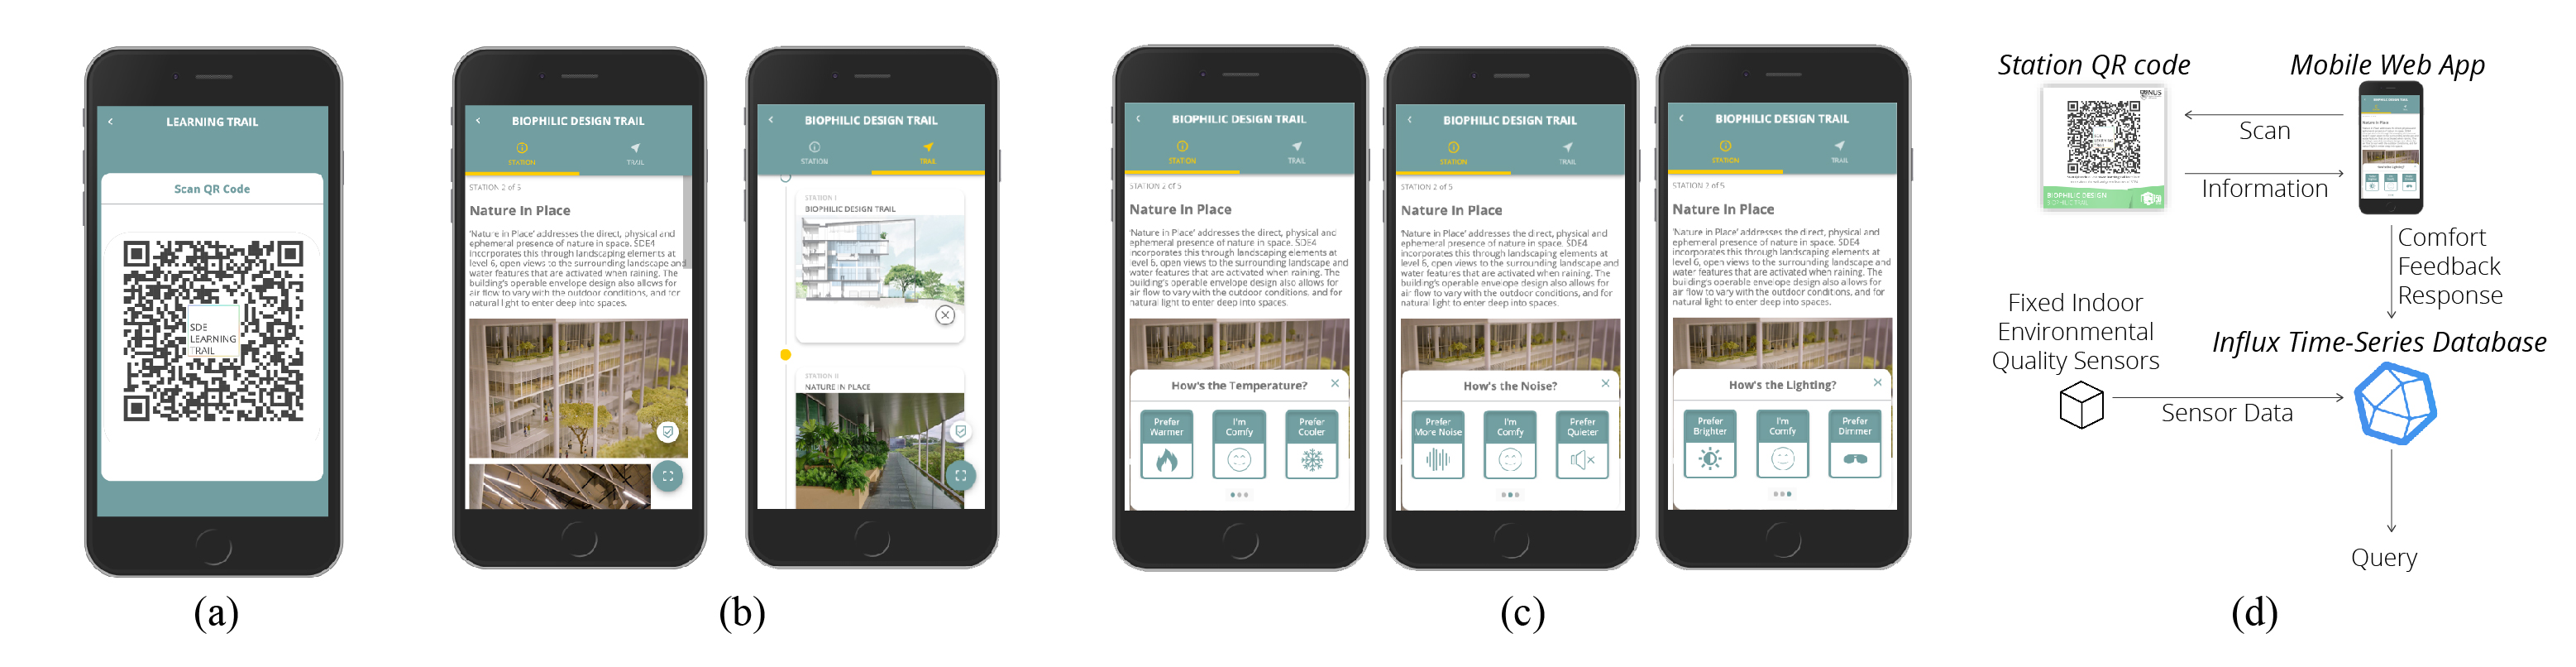
\includegraphics[width=\textwidth, trim= 0cm 0cm 0cm 0cm,clip]{Fig2.jpg}
\caption{Overview of Experiment Setup. (a) Biophilic Design trail as an example of trail placement in the building, (b) Photos from guided tours for participants, (c) Feedback prompts in the application, (d) Overview of data communication.}
\label{fig:experiments}
\end{center}
\end{figure}



\section{Results}
\label{ch:results}
% !TEX root = 99_main.tex

For the purposes of this publication, only an initial analysis of the collected environmental quality preference data is provided. The emphasis is to apply an unsupervised clustering technique to the occupant data to segment the users who provide more than five feedback points into cohorts of similar behavior. This type of analysis is the foundation for further research studies that characterize comfort preferences in ways that are specific to each occupant, but generalizable by grouping similar preference behavior. This particular analysis focuses on the behavior of each user in their interaction with the system instead of the demographic, physiological, or environmental conditions variables that are typically addressed in environmental preference studies. The aspects will be evaluated in future research. 

\subsection{Discovering occupant personal comfort preferences}
 
As shown in Figure \ref{fig:clustering}, five distinct clusters can be observed based on differences in preferences for temperature, light and noise levels across users. Predominantly users were comfortable and seldom preferred a change to cooler or quieter environments. Its interesting to discover differences in user \emph{preference personality types} based on the clustering. For instance, type \emph{A} prefers quieter spaces as compared to others, whereas \emph{B} prefers quieter surroundings. Type \emph{C} prefers bright and cool spaces, type \emph{D} is mostly comfortable with any condition and type \emph{E} prefers a mix of conditions, adjusting preferences but mostly comfortable with light levels. Understanding and defining these differences between user types can be used to personalize spatial recommendations to individual users based on their past preferences. Its important to note that Individual user feedback was clustered using unsupervised learning techniques. We used Ward's method for hierarchical clustering based on euclidean distance. 


%our approach for clustering individual user preferences for this analysis - though we used Ward's method for hierarchical clustering but changed to euclidean distance. 

%Its important to note that we slightly changed our approach for clustering individual user preferences for this analysis - though we used Ward's method for hierarchical clustering but changed to euclidean distance.

%As shown in Figure \ref{fig:clustering}, 5 distinct clusters can be observed based on differences between preferences for temperature, light and noise levels across users. Most  users were comfortable even in outdoor spaces, but sometimes would prefer cooler and quieter surroundings.\\

%Its interesting to discover differences in user "types" based on the clustering. For instance, type "A" users were 70-85\% of the time visually and thermally comfortable but only 30-45\% of the time aurally comfortable in the building. On the other hand, type "R" users were 85-100\% visually and aurally comfortable but 35-50\% thermally comfortable. Understanding and defining these differences between user types can be used to personalize spatial recommendations to individual users based on their past preferences.\\ 

%\subsection{Overview of the feedback data}

%Figure \ref{fig:feedbackdata}a shows the distribution of feedback votes between indoor and outdoor spaces. It's interesting to note that most feedback votes have been collected at outdoor stations in the trail. Limited nudging of users to provide feedback to avoid feedback fatigue \cite{EffectsFeedbackFatigue} and controlled access to participants for stations within indoor spaces are some of the reasons for this distribution.\\


%The locations of outdoor stations are naturally ventilated but shaded due to the building's large, overarching roof and open design. These environmental conditions had an effect on the feedback received as shown in Figure \ref{fig:feedbackdata}b. As shown, the figure provides a summary of all feedback vote categories for Temperature, light and noise variables. Its important to note that certain categories were less favored than others due to the feedback majority being gathered from outdoor stations. For instance, "Prefer Warmer" in temperature responses, and "Prefer Louder" in the noise responses were considerably less employed by the participants as compared to others in the same category due to tropical weather conditions and urban context of the building site.    


% \begin{figure}
% \begin{center}
% \includegraphics[width=\textwidth, trim= 0cm 0cm 0cm 0cm,clip]{Fig3.jpg}
% \caption{Overview of Feedback Data: (a) Split between outdoor vs. indoor feedback data (b) Correlation between spatio-temporal variables in indoor spaces (c) Correlation between spatio-temporal variables in outdoor spaces (d) Distribution of votes between temperature, light and noise variables.}
% \label{fig:feedbackdata}
% \end{center}
% \end{figure}


%\subsection{Correlations between spatio-temporal variables}

%Figure \ref{fig:feedbackdata}b shows correlations between different spatio temporal attributes for indoor and outdoor spaces.

%Figure \ref{fig:feedbackdata}b\&c shows that the relationship between "noise levels" and "presence" between indoor and outdoor spaces is reversed. This can be explained by the difference in primary noise source between the two space types - for indoor spaces the building occupants were the primary noise source, whereas for outdoor spaces thit was e surrounding urban context.\\

%Another interesting converse relationship is between "light levels" and "temperature" for indoor and outdoor spaces. An increase in light levels led to an increase in temperature for indoor spaces, whereas for outdoor spaces this effect could have been mitigated due to external environmental factors such as wind and humidity levels.\\



%\subsection{Distinguishing spaces based on comfort profiles}
%\label{ch:userResults}

%<<<<<<< HEAD
%Individual user feedback was clustered using unsupervised learning techniques. We used Ward's method for hierarchal clustering based on standardized euclidean distance.\\
%=======
%Individual user feedback was clustered using un-supervised learning techniques. We used Ward's method for hierarchical clustering based on standardised euclidean distance.\\
%>>>>>>> fc1014ad48bf8d01611951d862ceba4c900f2c56

%The results, shown in Figure \ref{fig:clustering}a, show 8 distinct clusters for comfort profiles of spaces based on user feedback. It can be observed that spaces are most frequently perceived as "comfy" or comfortable followed by preferences for more cooling and less noise. This pattern is reflective of majority of the feedback collected from outdoor spaces as noted before.\\

%It is important to recognize that unique profiles for spaces can be identified based on user's comfort perception of temperature, light and noise conditions. For instance, space cluster "A" is 40-50\% of the time thermally and aurally comfortable and 80\% or more visually comfortable. On the other hand, space cluster "F" is perceived 80-100\% thermally, aurally, visually comfortable most times.         


  


\begin{figure}
\begin{center}
\includegraphics[width=\textwidth, trim= 0cm 0cm 0cm 0cm,clip]{Images/Fig3.jpg}
\caption{Indoor and outdoor comfort preference clustering: Users are grouped based on comfort preferences: A) Prefers quieter spaces compared to others, B) Prefers cooler and quieter spaces, C) Prefers brighter and cooler spaces, D) Mostly comfortable, E) Preferences of this type keep changing as compared to others but they are usually comfortable with light levels}
\label{fig:clustering}
\end{center}
\end{figure}




\section{Discussion}
\label{ch:discussion}
% !TEX root = 99_main.tex

\subsection{Choice of a field based experiment setup}
The goals for conducting comfort assessments under controlled lab settings can be different from conducting the same in field conditions. The former is better suited for dispositional approaches - where the surrounding environment doesn't effect participant behavior, whereas the latter is focused on situational approaches - where behavior is dependent on the surrounding context.
Given that the one of the aims for this study was to understand the dynamic nature of occupant comfort in different environmental and spatial contexts, the research team chose a field based experiment setup to provide higher ecological validity to the findings compared to a lab experiment \cite{andrade2018internal}.           


\subsection{Findings from large data and a 3-point scale}
%\label{ch:localisation}

Generalizing findings for the larger population using detailed surveys or interview results from a small group of participants was a trusted method for comfort assessments in building research in the past. However with new technologies and modern data capabilities, collection, processing and analysis of large data sets has become easier. That's why this study utilizes QR codes, an interactive mobile application and time-series database infrastructure to collect and process a relatively large comfort assessment data set in a short time. As highlighted earlier in Section \ref{ch:introduction}, comfort feedback data can be skewed due to a participant's personal traits, geographical and cultural background and response biases. To limit subjectivity and make it easy for participants to provide feedback in field conditions, the team used a 3-point comfort scale rather than the traditional 7-point comfort scale. This not only saved participant's effort and time in the field but also helped channelize and organize data streams for the research team easily.

% It's interesting to reflect upon the kind of conclusions that can be derived as a result. The traditional method can derive detailed conclusions such as "5 of the 20 users felt comfortable at temperatures lower than 22 $^\circ$C". Whereas the large data method can draw conclusions such as "5 of 20 users can be categorized as a user type that prefers cooler working environments". 


\subsection{Identification of occupant types}

This study identifies personalized comfort profiles of users through data driven methods - which basically cluster users into \emph{types}. This could be used to understand, and even predict, patterns and anomalies in occupant behavior and occupant profiling in the future. Its easy to see how the same methodology could be used to distinguish spaces based on occupant comfort feedback data - to derive comfort profiles of spaces.


\subsection{Limitations}
It is important to note that the SDE4 building is operational, but still under a defect and liability period. Since a majority of the new building's systems are still undergoing calibration and refinenement for full operations in the future, multiple data sources are not integrated into this analysis. This analysis is preliminary and further convergence of data from these other sources such as fixed environmental sensors, demographic information, and physiological information from wearable devices will produce more traditional comfort modeling insight. Additionally, given nature of use of this application for orientation tours of SDE4, users are most likely to participate only once. While this constraints the comparison of occupant comfort feedback and spatio-environmental variables over time for each participant - at the end of the tour, participants are pointed to an advanced spatial recommendation application which uses their comfort feedback to match them to suitable spaces in the building for flexible working. More nuanced occupant feedback and spatial-environmental data is collected for participants which use these flexible workspaces over time. More details regarding the spatial recommendation system and its application would be provided in a future publication.











\section{Conclusion}
\label{ch:conclusion}
% !TEX root = 99_main.tex

This paper describes the pilot implementation of Learning Trail application at the new building in NUS for occupant comfort data collection. Within just three months, 1163 environmental feedback momentary assessment surveys of thermal, visual and aural comfort were obtained participants who gave five or more votes. A total of 616 participants have contributed to the study till date, with minimal administrative overhead. This rich data set provides new opportunities for understanding occupant comfort behavior through data driven methods. Within this study, we've demonstrated how data can be used to group occupants into comfort profile types and shown this study as potential stepping stone to other research areas such as comfort profiling of spaces, occupant behavior analysis and correlation identification between various spatiotemporal variables in buildings. 
Segments of the raw data and analysis code used in this analysis will be available in an open-access Github repository that includes documentation on the Learning Trail app\footnote{\url{https://github.com/buds-lab/cisbat-learning-trail-paper}}. The app is a mobile, web-based platform that can be deployed in other locations in collaboration with the authors.

% As a logical next step, this study provides the proof of concept for the complimentary SpaceMatch project - a spatial recommendation system that utilizes the collected data from this study to match user comfort profiles to spaces that best suit them in real time.

% \subsection{Reproducibility}





% \section{Acknowledgments}
% \label{ch:acknowledgments}
% % !TEX root = 99_main.tex

The authors would like to acknowledge the HiLo and HoNR project members for the design and construction of the ASF: Supermanoeuvre (Sydney Australia) and the Professorship of Architecture and Structures (BRG, ETH Zurich) for their work in designing the HiLo building; and the Institute of Structural Engineering (IBK, ETH Zurich) for their work in designing the HoNR building. The authors would also like to thank other key contributors to the ASF Project: Bratislav Svetozarevic, Moritz Begle, Stefan Caranovic. \\

This research was partly funded by the Climate-KIC, Building Technologies Accelerator program.


% \begin{appendices}
%  \label{ch:appendix}
%  % !TEX root = 99_main.tex

%  \end{appendices}

%% appendix sections are then done as normal sections
%% \appendix
%% \section{}
%% \label{}

%% bibitems, please use
\section*{References}
  \bibliographystyle{elsarticle-num} 
  \bibliography{references}

\end{document}
\endinput
